\documentclass[9pt, conference, a4paper, compsocconf]{IEEEtran}
\usepackage{amsmath,amsxtra,amssymb,amsthm,latexsym,amscd,amsfonts}
\usepackage{iftex}
\ifXeTeX\usepackage{fontspec}\setmainfont{Times New Roman}\else\usepackage[utf8]{vietnam}\fi
\usepackage[top=2.7cm, bottom = 5.4cm, left=2.72cm, right = 2.85cm]{geometry}
\headsep = 0.7cm
\headheight = 1.0cm 
\footskip = 1.0cm
\voffset = -0.74 cm 
%%%%
\usepackage{balance}

\usepackage{fancyhdr}
\pagestyle{fancy}
\usepackage{cite}
\usepackage{algorithmic}
\usepackage{graphicx}
\usepackage{textcomp}
\usepackage{booktabs}   
\usepackage{tabularx}  
\usepackage{xcolor}
\usepackage{amsmath,amsxtra,amssymb,amsthm,latexsym,amscd,amsfonts}
\usepackage{pgfplots}
\usepackage{multirow}
\usepackage{subcaption}
\pgfplotsset{compat=1.17} 

\usepackage{tikz}
\usetikzlibrary{positioning}  
\usetikzlibrary{arrows.meta}  
\usetikzlibrary{shapes}      
\usetikzlibrary{calc}      
\usetikzlibrary{fit}          
\usepackage[english]{babel} %Figure ... English (có thể bỏ đi nếu bài viết tiếng Việt)
\usepackage{fancyhdr}
\pagestyle{fancy}
%\renewcommand{\chaptermark}[1]{\markboth{\MakeUppercase{#1}}{}}
\renewcommand{\sectionmark}[1]{\markright{\MakeUppercase{#1}}{}}
\renewcommand{\headrulewidth}{0pt}
\DeclareGraphicsExtensions{.pdf,.jpeg,.png,.jpg}

\usepackage{array}

\usepackage{caption}
\captionsetup{
  font={footnotesize}, 
  justification=centering,
  singlelinecheck=false
}

\makeatletter
\def\ps@IEEEtitlepagestyle{%
\def\@oddhead{\hfil \small{\textit{Hội thảo khoa học Quốc gia về Trí tuệ nhân tạo 2027 (FJCAI) - Đà Nẵng, 8-9/4/2027}\hfil}%
	\def\@evenhead{\hfil\small{\textit{Hội thảo khoa học Quốc gia về Trí tuệ nhân tạo 2027 (FJCAI) - Đà Nẵng, 8-9/4/2027}\hfil}}%
		\def\@oddfoot{\scriptsize \thepage \hfil }%
		\def\@evenfoot{\scriptsize \hfil \thepage}
	}
}

\def\@maketitle{%
  \newpage
  \null
  \begin{center}%
    {%
      \fontsize{16}{18}\selectfont
      \bfseries \@title \par
    }%
    \vskip 4em%
    {%
    \fontsize{9}{3.5}\selectfont
      
      \begin{tabular}[t]{c}%
        \@author
      \end{tabular}\par
    }%
  \end{center}%
  \par
}

\renewenvironment{abstract}
  {\normalfont
   \if@twocolumn
     \@IEEEabskeysecsize\bfseries\textit{\abstractname}: 
   \else
     \begin{center}\@IEEEabskeysecsize\textbf{\abstractname}\end{center}
     \@IEEEabskeysecsize
     \setlength{\parindent}{0pt}   % ← tắt thụt đầu dòng
     \noindent
   \fi}
  {\par}

\renewenvironment{abstract}
  {\normalfont
   \@IEEEabskeysecsize
   \setlength{\parindent}{0pt}
   \noindent
   \if@twocolumn
     \bfseries\textit{\abstractname}: 
   \else
     \begin{center}\textbf{\abstractname}\end{center}
   \fi}
  {\par}
  
\renewenvironment{IEEEkeywords}
  {\normalfont
   \@IEEEabskeysecsize
   \vspace{0.3em}       
   \setlength{\parindent}{0pt}
   \noindent
   {\bfseries\itshape \IEEEkeywordsname: }\ignorespaces}
  {\par}

\def\IEEEbibitemsep{1.5pt plus .5pt}

\makeatother



\makeatletter
\AtBeginDocument{
  \renewcommand{\abstractname}{Tóm tắt}
}
\renewcommand{\IEEEkeywordsname}{Từ khóa}
\makeatother



\begin{document}
\pagenumbering{gobble}
\fontsize{9}{10}
\selectfont

\fancyhead[RE,LO]{\centering{\small{\textit{Hội thảo khoa học Quốc gia về Trí tuệ nhân tạo 2027 (FJCAI) - Đà Nẵng, 8-9/4/2027}}}}


% end of customization

%
\title{M2G-NET Under Eligibility and Partial Labels:\\A Synthetic Audit}

% Author identity as supplied by the user in P28 (docs/paper/task-notes/P28.md).
% Anonymity requirement of FJCAI 2027 is unverified; blank this block if double-blind is required.
\author{\IEEEauthorblockN{Đặng Tuấn Kiệt}
	\IEEEauthorblockA{Smart Green Transformation Center (Green-X)\\
	Email: 25kiet.dt@vinuni.edu.vn}
}

\maketitle

\begin{abstract}
Multi-task prediction can combine related outcomes while obscuring differences in outcome eligibility, label observation and the populations actually scored. Transport-motivated endpoints illustrate the problem: red-light behavior is defined for a red-phase encounter and turn-signal behavior for a turning rider, and an ineligible outcome must not be coded as an observed negative. This study audits M2G-NET, a categorical multi-view model combining individual-context interactions, task-specific gated fusion and masked multi-task learning, and evaluates the implemented model against other model families instead of assuming it helps. The contribution is an auditable simulation and evaluation design, not a new gate, a new masking principle or an empirical motorcycle-behavior finding. An architecture-independent generator specifies additive, interaction and partial-observation mechanisms with 3,000 encounters at 12 fixed sites and four synthetic binary endpoints. Ten independent generator replicates per mechanism (three prespecified, seven added post hoc after the first three were examined) and two training seeds give 300 fits of five procedures: M2G-NET, an independent-head MLP, a shared one-hot MLP, one-hot logistic regression and CatBoost. Full-model mean macro AUC was 0.626 on additive data, 0.740 on interaction data and 0.741 on partial-label data. On interaction and partial-label data the full model was ahead of the independent-head MLP and of logistic regression on all ten datasets, and ahead of CatBoost on nine and eight of ten. Logistic regression was best on the additive control, and other procedures achieved lower Brier error. The results are descriptive, synthetic and conditional on fixed sites; they do not establish architectural improvement, statistical significance or real-world transport benefit.
\end{abstract}

\begin{IEEEkeywords}
\textbf{\textit{multi-task learning; gated fusion; simulation study; partial labels; outcome eligibility
}}
\end{IEEEkeywords}

\IEEEpeerreviewmaketitle

\section{Introduction}
Motorcycle safety is a setting in which several outcomes may be recorded for the same encounter while their applicability differs. An observational study of delivery, ride-hailing and private riders in Hanoi evaluated red-light behavior among red-phase encounters and turn-signal behavior among turning riders \cite{NguyenPhuoc2024same}. This motivates careful handling of outcome eligibility. It does not give the present study individual records, and it does not show that generated outcomes reproduce rider behavior.

We take a simulation-methods route with four synthetic binary endpoints that carry transport-motivated names and categorical input groups. An ineligible endpoint must not become an observed negative, and an eligible but missing label must remain distinguishable from both a negative and ineligibility. This fixes which population an evaluation scores. It does not identify a real missing-data process \cite{RUBIN1976inference}.

Learned sharing is an established topic: Cross-Stitch networks, task-specific expert gates in MMoE and progressive extraction in PLE all precede this work \cite{Misra2016cross,Ma2018modeling,Tang2020progressive}. M2G-NET combines view-specific encoders, an individual-context interaction block, task-specific gated fusion, a shared early-fusion path and a masked objective. Feature crossing, uncertainty-based loss weighting and normalized task-specific losses also have precedents \cite{Wang2017deep,Kendall2018multi,Tang2020progressive}. The question is therefore how this documented implementation behaves under stated data-generating mechanisms, not whether its parts have existed before. Our bounded literature check does not establish that the combination is unique.

\textbf{Research question.} Under synthetic mechanisms with grouped categorical views and partially observed eligible binary outcomes, when does the implementation improve, match or degrade performance relative to simpler procedures? Following structured simulation reporting \cite{Morris2019using}, generator design, denominators and the first three replicates per mechanism were fixed before final evaluation, and a favorable result was not assumed. The replication count was later extended post hoc, as disclosed below.

\textbf{Contributions.} (i) An implementation description checked against equations and code. (ii) An architecture-independent, reproducible simulation specification with separate predictor and oracle artifacts. (iii) Frozen-procedure comparisons that include negative results and per-task trade-offs. The scope excludes real rider behavior, causal explanation, fairness certification, policy advice and unseen-site generalization.

\section{Related Work}
\textit{Shared representations and routing.} Caruana frames multi-task learning as inductive transfer through shared representations learned from related tasks \cite{Caruana1997multitask}. This supports studying sharing, not assuming that sharing improves arbitrary outcomes. Cross-Stitch networks learn linear combinations of task activation maps, a precedent for learning how representations are shared rather than fixing every shared/task-specific boundary \cite{Misra2016cross}; their convolutional vision setting differs from the categorical views and input-dependent routing considered here. MMoE shares expert networks and uses a separate gate for each task, and its author abstract describes experiments varying task relationships, including synthetic tasks \cite{Ma2018modeling}. Task-specific gates and synthetic task-relationship experiments therefore do not originate with M2G-NET. Our check verifies that abstract, not an unread equation or result in the full paper. Naming both systems gated does not establish architectural equivalence: here, separate encoders represent predefined views.

PLE separates shared and task-specific expert components with progressive routing, and discusses cases in which one task improves while others deteriorate \cite{Tang2020progressive}. This motivates reporting per-task comparisons alongside macro summaries.

\textit{Recent developments.} Research on routing and sharing is still active. ETR-NLP mitigates task interference with explicit shared and task-specific branches and reports gains over baselines on image classification and dense prediction \cite{Ding2023mitigating}. BEnet addresses a polarization problem in MMoE, in which some expert weights converge towards zero, and reports gains on real-world datasets \cite{Zhang2025bagging}. These works target vision and recommendation settings and are evaluated on their own benchmarks; they motivate checking a routing design against simpler references but do not transfer to the present categorical, eligibility-masked setting. Joint-Task Regularization addresses data that are not fully labeled for all tasks by regularizing tasks in a joint latent space \cite{Nishi2024joint}; our masked loss instead leaves missing targets out and does not use cross-task regularization. In transport safety, a recent multi-task framework predicts several crash-severity targets from multi-source data \cite{Xiao2025explainable}, which shows applied interest in multi-target prediction but not a controlled evaluation of eligibility and observation.

\textit{Interactions and objectives.} Sparsemax is an established projection-based alternative to softmax \cite{Martins2016from}. Focal loss modulates cross-entropy by prediction difficulty \cite{Lin2017focal}; the implementation here uses a symmetric scalar multiplier, not the original class-balanced variant. Deep\,\&\,Cross Network combines a deep branch with explicit feature-crossing layers that construct bounded-degree interactions \cite{Wang2017deep}. This establishes prior explicit crossing of encoded features, not equivalence to M2G-NET's projected individual-context products. Kendall \emph{et al.} derive task-loss weighting from homoscedastic uncertainty \cite{Kendall2018multi}; M2G-NET uses an adapted scale-weighted surrogate on observed-label-normalized losses, not an identical Bernoulli likelihood or a calibrated uncertainty estimate.

\textit{Partial labels and evaluation populations.} PLE includes an indicator-normalized loss that excludes samples outside a task's sample space \cite{Tang2020progressive}, so masked normalized training is prior art. Task ineligibility and an unobserved eligible label are different states. Ignoring an observation process requires conditions appropriate to the inferential setting \cite{RUBIN1976inference}, and a mask in a neural loss does not establish them or recover an unidentified outcome-dependent process. In a generated study, eligibility, observation probabilities and latent eligible labels can be specified separately; their role is to define and evaluate a controlled estimand, not to pretend that a real observation process has been identified.

\textit{Transport motivation and simulation reporting.} The rider study motivating the feature groups uses different applicable populations for red-light and turn-signal outcomes \cite{NguyenPhuoc2024same}. This motivates explicit synthetic endpoint definitions and event masks; it does not authorize using its raw records or transferring observed associations. Morris \emph{et al.} organize simulation studies by aims, data-generating mechanisms, estimands, methods and performance measures, and stress uncertainty from finite repetitions \cite{Morris2019using}. We follow that logic and separate generator replicates from training seeds; following guidance does not establish adequate precision for any chosen replication count. A review of 321 simulation-methods articles found that many omit a justification for the number of repetitions, Monte Carlo uncertainty estimates, or code and data \cite{Siepe2024simulation}; we report the replication count with Monte Carlo standard errors of the means, which do not by themselves make that count adequate. Declaring a plan before outcomes are known is argued to reduce bias and improve transparency \cite{Hardwicke2023reducing}; we claim no public registration. This supports only a restrained positioning: evaluate an audited integration and report advantages, parity and failures, without claiming uniqueness or transfer to deployment.

\section{Method}
This section describes the existing implementation that was audited against its code and used in the frozen evaluation.

\subsection{Views and encoders}
An encounter has five categorical views: rider role, rider traits, road context, environment and observed site infrastructure. A site identifier indexes a learned site representation. Four heads correspond to the red-light, turn-signal, helmet and phone synthetic endpoints; the names label synthetic targets, not recoded observational categories. Each feature has an eight-dimensional embedding. Within a view, embeddings are concatenated and passed through a width-32 affine layer, ReLU, dropout 0.3 and an affine layer to $h_j\in\mathbb{R}^{16}$. Vocabularies are fitted on training rows with unknown-category handling. The site view concatenates an infrastructure encoding $h_{obs}$ with a 16-dimensional site embedding $e_s$:
\begin{equation}
h_{site}=\mathrm{ReLU}(W_s[h_{obs};e_s]+b_s).
\end{equation}
The unknown site has $e_s=0$. This is a regularized intercept-like representation, not a mixed-effects model.

\subsection{Individual-context interaction}
With $h_{ind}\in\mathbb{R}^{32}$ (role and traits) and $h_{ctx}\in\mathbb{R}^{48}$ (road, environment, site), let $p_{ind}=W_{ind}h_{ind}+b_{ind}$ and $p_{ctx}=W_{ctx}h_{ctx}+b_{ctx}$. Then
\begin{align}
u&=p_{ind}+p_{ctx}+W_{int}(p_{ind}\odot p_{ctx})+b_{int},\\
h_{int}&=\mathrm{Dropout}\{\mathrm{GELU}(W_ou+b_o)\}.
\end{align}
All projected vectors have dimension 16. A fitted weight here does not identify a causal interaction.

\subsection{Gated fusion and residual blending}
An affine map of $h_{int}$ gives $v_6$; with the five view vectors $v_1,\dots,v_5$, set $r=[v_1;\dots;v_6]$. For task $k$,
\begin{align}
\tilde a_k&=\mathrm{sparsemax}\big((A_kr+c_k)/\max(T,0.1)\big),\\
a_k&=(1-\lambda)\tilde a_k+\lambda\mathbf{1}/6,
\end{align}
with $\lambda=0.1$, so every final weight is at least $0.1/6$ and the smoothed gate is not exactly sparse. The temperature $T$ follows a schedule and is not learned. The gated representation is $z_{gated,k}=\sum_j a_{kj}v_j$. A shared early-fusion MLP on the five original views (widths 80, 32, 16) gives $z_{early}$. A single learned scalar $b$, initialized so that $\sigma(b)=0.5$, blends the paths:
\begin{equation}
\begin{split}z_k&=\sigma(b)z_{gated,k}+[1-\sigma(b)]z_{early},\\ \hat y_k&=\sigma(w_k^{\top}z_k+d_k).\end{split}
\end{equation}
Fig.~\ref{fig:arch} summarizes the architecture. Gates describe model allocation, not causal importance.

\begin{figure}[t]
\centering
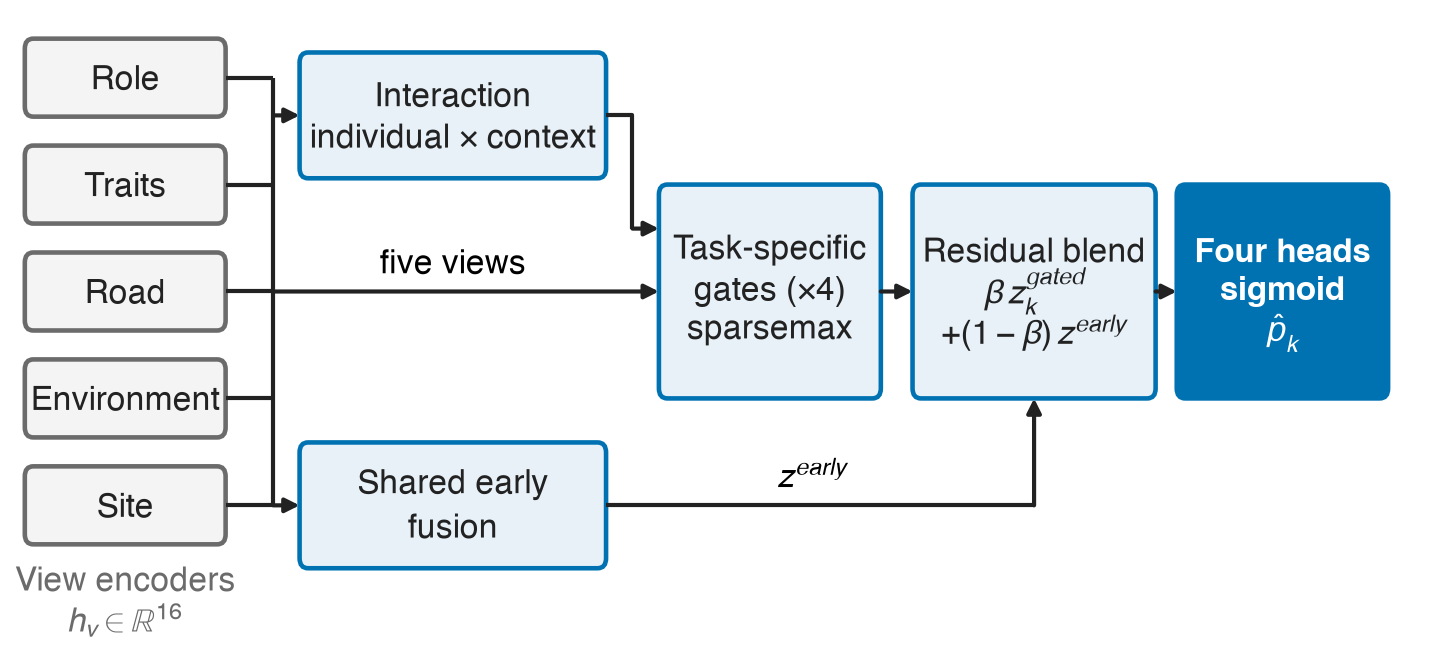
\includegraphics[width=\columnwidth]{figures/fig1_architecture.png}
\caption{M2G-NET: five view encoders, an individual-context interaction block, four task-specific sparsemax gates, a shared early-fusion path and a residual blend feeding four sigmoid heads.}
\label{fig:arch}
\end{figure}

\subsection{Eligible and observed outcomes}
For encounter $i$ and task $k$, let $E_{ik}$ indicate eligibility, $R_{ik}$ observation among eligible outcomes and $M_{ik}=E_{ik}R_{ik}$ the training mask. Targets with $M_{ik}=0$ are indexed out before the binary loss is computed, so a missing target is never converted into an observed negative. The loss receives $M$ and does not infer $E$ or $R$; correct eligibility must come from the generator or an authorized codebook.

\subsection{Objective and optimization}
For an observed outcome let $p_t=\hat y$ if $y=1$ and $1-\hat y$ otherwise. The base loss is a scalar-rescaled focal form, with the same factor 0.25 for both classes:
\begin{equation}
\ell_{ik}=0.25(1-p_t)^2\,\mathrm{BCE}(\hat y_{ik},y_{ik}),\quad
\bar\ell_k=\frac{\sum_iM_{ik}\ell_{ik}}{\sum_iM_{ik}}.
\end{equation}
For tasks observed in the mini-batch, with $s_k=\log\tau_k^2$,
\begin{equation}
\mathcal{L}=\sum_{k:\sum_iM_{ik}>0}\Big[\tfrac12e^{-s_k}\bar\ell_k+\tfrac12s_k\Big].
\end{equation}
A task with no observed outcome contributes neither term. This is adapted from \cite{Kendall2018multi} and is not an exact Bernoulli likelihood or calibrated uncertainty. Training uses Adam \cite{Kingma2015adam} (learning rate 0.001, weight decay 0.0001, batch 64), cosine schedules, gradient clipping at norm 1 and validation macro-AUC checkpoint selection.

\section{Simulation Design}
\subsection{Mechanisms}
Each dataset has 3,000 encounters at 12 fixed sites, 250 per site. For site $s=0,\dots,11$, signal presence is Yes if $s<8$, lanes are $2+(s \bmod 3)$ and the intersection is Cross for even $s$. Task $k=0,\dots,3$ has site offset $u_{sk}=0.25\sin(2\pi(s+1)(k+1)/13)$. Within a site, features are drawn independently from fixed categorical laws (rider type 0.30/0.30/0.40, gender 0.40/0.60, age 0.35/0.45/0.20, police 0.70/0.30, traffic 0.25/0.45/0.30, weather 0.80/0.20, peak 0.50/0.50, weekend 0.70/0.30). These are design choices, not estimates from the Hanoi study. With the coded predictor vector $x_i$ and fixed task coefficient vectors $B_k$, the additive mechanism uses $\eta_{ik}=x_iB_k+u_{sk}$. The interaction mechanism adds $G_k(rt,\,ap,\,rw)$, products of rider type with traffic, age with police and rider type with weather. Outcomes are $Y_{ik}=\mathbf{1}[U_{ik}<\sigma(\eta_{ik})]$. The full coefficient tables are in the artifact inventory, not reproduced here.

\subsection{Eligibility and partial observation}
Fig.~\ref{fig:elig} summarizes the outcome states. A red-phase encounter occurs with probability 0.75 at signalized sites and zero elsewhere; a turn occurs with probability 0.70. These define red-light and turn-signal eligibility, and helmet and phone are always eligible. Oracle outcomes are absent where $E=0$. Additive and interaction mechanisms observe every eligible outcome. The partial mechanism keeps the interaction outcome law and observes an eligible label with probability
\begin{equation}
\rho_{ik}=0.75+0.20\,\sigma(C_k+0.5r-0.4t+0.3q+0.2g),
\end{equation}
so $0.75<\rho<0.95$, with $C=(-0.40,-0.10,0.20,0.40)$. This is one covariate-dependent process and not a remedy for arbitrary informative missingness. The predictor export contains configured features, site ID, observed labels, masks and non-predictor audit flags only. Latent eligible outcomes, probabilities and observation propensities stay in a separate oracle file that never reaches fitting or validation selection. Independent generator seeds are 1701--1703 (prespecified) and 1704--1710. The latter seven were added after the first three replicates had been examined, to check whether their ordering was stable; they reuse the frozen commands, hyperparameters and scorer unchanged. The extension is therefore post hoc, and all ten replicates are reported. Development seed 1601 is excluded from all results.

\begin{figure}[t]
\centering
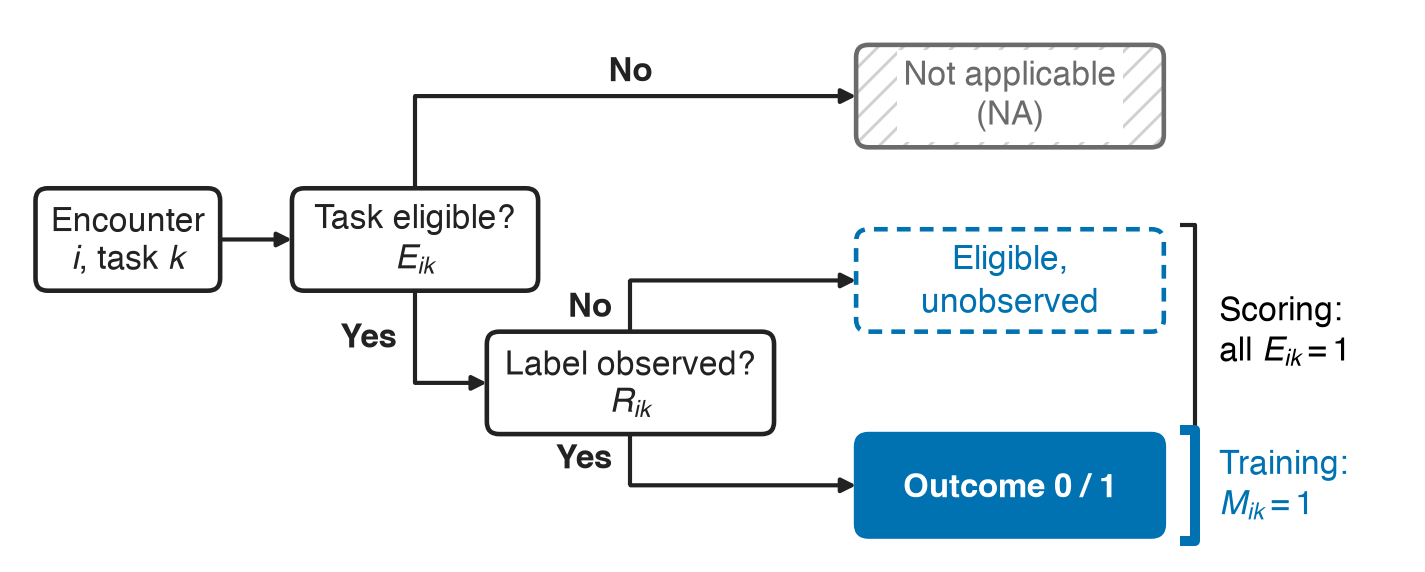
\includegraphics[width=\columnwidth]{figures/fig2_eligibility.png}
\caption{Outcome states for encounter $i$ and task $k$. Ineligible outcomes ($E=0$) are not applicable, not negatives. Eligible outcomes are observed ($R=1$) or unobserved ($R=0$). Training uses observed outcomes ($M=E\times R=1$); primary evaluation scores all eligible outcomes against oracle labels.}
\label{fig:elig}
\end{figure}

\subsection{Procedures and selection}
Procedures are M2G-NET, an independent-head MLP, a shared one-hot MLP, one-hot logistic regression and categorical CatBoost \cite{Prokhorenkova2017catboost}. All predict the same outer test rows within a dataset. The 70/10/20 split uses seed 42 and a label-signature stratifier; it is not outcome-blind. Training seeds 42 and 101 are repeated in every dataset. Neural fits use at most 150 epochs with patience 20. Logistic regression selects $C\in\{0.1,1,10\}$ and CatBoost depth in $\{4,6,8\}$, per task. Classical procedures thus have three candidates per task and neural procedures one configuration; these are not equal-capacity or equal-search comparisons. A large benchmark of 19 algorithms on 176 tabular datasets found that, for many datasets, light tuning of a boosted-tree model mattered more than the choice between neural and tree models \cite{McElfresh2023when}, so differences in search budget here are a first-order caveat.

\subsection{Endpoints and aggregation}
The primary endpoint is raw-probability ROC-AUC on all eligible held-out outcomes, including eligible outcomes masked from fitting. Four task AUCs are averaged equally. An undefined task AUC would invalidate that macro value, and none occurred. Secondary endpoints are average precision (AP) and Brier score. Training seeds are averaged within dataset, then ten independent datasets are summarized by mean, sample SD, range, Monte Carlo standard error (SD/$\sqrt{10}$) and the number of datasets with a positive paired difference. There are no significance tests or population confidence intervals. For the three original replicates, AUC and squared error were independently recomputed during the audit; the extension reuses the same scorer, reproduces the original rows exactly and was not separately recomputed.

\section{Results}
All 300 fits completed over 30 datasets (600 test encounters each) and every eligible task test set contained both classes. Partial-label red-light eligibility ranged from 285 to 323 test encounters, of which 237--279 were observed. Tables~\ref{tab:macro} and~\ref{tab:cost} summarize the outcomes.

\begin{table*}[t]
\caption{Macro performance on eligible test outcomes: mean over ten generated datasets, each averaged over two training seeds. Bold: best per mechanism and metric (ties at three decimals both bold). Higher AUC and AP, lower Brier are better.}
\label{tab:macro}
\centering\footnotesize
\begin{tabular}{lccccccccc}
\toprule
 & \multicolumn{3}{c}{Additive} & \multicolumn{3}{c}{Interaction} & \multicolumn{3}{c}{Partial} \\
\cmidrule(lr){2-4}\cmidrule(lr){5-7}\cmidrule(lr){8-10}
Procedure & AUC & AP & Brier & AUC & AP & Brier & AUC & AP & Brier \\
\midrule
M2G-NET & 0.626 & 0.478 & 0.230 & \textbf{0.740} & \textbf{0.641} & 0.212 & \textbf{0.741} & \textbf{0.643} & 0.211 \\
Independent MLP & 0.628 & 0.479 & 0.219 & 0.725 & 0.628 & 0.201 & 0.726 & 0.626 & 0.200 \\
Shared one-hot MLP & 0.627 & 0.478 & \textbf{0.218} & 0.734 & 0.636 & \textbf{0.198} & 0.736 & 0.636 & \textbf{0.197} \\
Logistic regression & \textbf{0.632} & \textbf{0.483} & \textbf{0.218} & 0.657 & 0.559 & 0.217 & 0.658 & 0.555 & 0.216 \\
CatBoost & 0.621 & 0.473 & 0.219 & 0.732 & 0.634 & 0.199 & 0.737 & 0.635 & 0.198 \\
\bottomrule
\end{tabular}
\end{table*}

\subsection{Additive control and interaction setting}
On additive data, M2G-NET reached 0.626 mean macro AUC (dataset SD 0.014), below logistic regression (0.632), the independent-head MLP (0.628) and the shared one-hot MLP (0.627).

In the interaction setting M2G-NET reached 0.740 (SD 0.008), compared with 0.657 for logistic regression, 0.732 for CatBoost and 0.734 for the shared one-hot MLP. Ranking and probability error disagreed: M2G-NET Brier was 0.212 against 0.198 for the shared one-hot MLP and 0.199 for CatBoost.

\textbf{Where the full model was consistently ahead.} Table~\ref{tab:paired} shows that the full-minus-comparator paired difference was positive on all ten generated datasets, for both interaction and partial-label data, against the independent-head MLP ($+0.0146$ and $+0.0150$ on average) and logistic regression ($+0.0832$ on both). Against the shared one-hot MLP it was positive on nine of ten datasets in each setting ($+0.0062$, $+0.0059$) and against CatBoost on nine of ten interaction datasets ($+0.0083$, minimum $-0.0019$), eight of ten partial-label datasets ($+0.0049$) and eight of ten additive datasets ($+0.0044$). Sign counts are not significance tests, and these comparators differ in capacity, preprocessing and search budget, so the comparison supports a procedure-level ordering, not credit to one module.

\textbf{Effect of the post-hoc extension.} In the first three replicates alone, the full model was ahead of CatBoost on every interaction dataset. With ten replicates this no longer holds: one interaction dataset favors CatBoost. We report the ten-replicate results as primary because three replicates gave unstable ranges, and the three-replicate tables remain in the artifact files.

\subsection{Partial observation}
With partial labels M2G-NET scored 0.741 (SD 0.013), against 0.726 for the independent-head MLP, 0.736 for the shared one-hot MLP, 0.737 for CatBoost and 0.658 for logistic regression.

\begin{table}[t]
\caption{Computational comparison (frozen runs). Parameters are trainable counts. Search: candidate fits per unit. Runtime: mean fit seconds.}
\label{tab:cost}
\centering\footnotesize
\begin{tabular}{lccc}
\toprule
Procedure & Params & Search & Runtime (s) \\
\midrule
M2G-NET & 14.3k & 1 & 14.3 \\
Independent MLP & 5.1k & 1 & 6.4 \\
Shared one-hot MLP & 4.7k & 1 & 6.2 \\
Logistic regression & n/a & 12 & 3.1 \\
CatBoost & n/a & 12 & 5.2 \\
\bottomrule
\end{tabular}
\end{table}

Table~\ref{tab:pertask} gives the per-task AUCs behind the macro averages and Table~\ref{tab:paired} the paired differences with their dataset-level ranges and positive counts; both retain every negative comparison. Fig.~\ref{fig:paired} shows the ten dataset-level deltas behind each mean, so sign changes across datasets are visible directly.

\begin{table*}[!t]
\caption{Per-task mean AUC on eligible test outcomes (ten generated datasets, two training seeds each). Negative comparisons are retained; no task is selected after the fact. RL: red-light, TS: turn-signal, HM: helmet, PH: phone.}
\label{tab:pertask}
\centering\footnotesize\setlength{\tabcolsep}{3pt}
\begin{tabular}{lcccccccccccc}
\toprule
 & \multicolumn{4}{c}{Additive} & \multicolumn{4}{c}{Interaction} & \multicolumn{4}{c}{Partial} \\
\cmidrule(lr){2-5}\cmidrule(lr){6-9}\cmidrule(lr){10-13}
Procedure & RL & TS & HM & PH & RL & TS & HM & PH & RL & TS & HM & PH \\
\midrule
M2G-NET & 0.656 & 0.615 & 0.621 & 0.611 & 0.724 & 0.727 & 0.758 & 0.750 & 0.740 & 0.725 & 0.754 & 0.747 \\
Independent MLP & 0.660 & 0.618 & 0.621 & 0.611 & 0.710 & 0.712 & 0.746 & 0.733 & 0.717 & 0.711 & 0.741 & 0.737 \\
Shared one-hot MLP & 0.663 & 0.615 & 0.622 & 0.610 & 0.721 & 0.718 & 0.755 & 0.741 & 0.724 & 0.727 & 0.745 & 0.746 \\
Logistic regression & 0.667 & 0.615 & 0.628 & 0.618 & 0.647 & 0.610 & 0.707 & 0.664 & 0.647 & 0.611 & 0.694 & 0.681 \\
CatBoost & 0.649 & 0.605 & 0.620 & 0.611 & 0.724 & 0.705 & 0.756 & 0.742 & 0.726 & 0.719 & 0.751 & 0.750 \\
\bottomrule
\end{tabular}
\end{table*}

\begin{table*}[!t]
\caption{Paired macro AUC differences, M2G-NET minus comparator (positive favors M2G-NET), over ten generated datasets: mean $\pm$ Monte Carlo standard error of the training-seed-averaged paired delta, dataset-level [min, max] and number of datasets with a positive delta. Descriptive only: no significance claim is made.}
\label{tab:paired}
\centering\scriptsize\setlength{\tabcolsep}{2.5pt}
\resizebox{\textwidth}{!}{%
\begin{tabular}{lccccccccc}
\toprule
 & \multicolumn{3}{c}{Additive} & \multicolumn{3}{c}{Interaction} & \multicolumn{3}{c}{Partial} \\
\cmidrule(lr){2-4}\cmidrule(lr){5-7}\cmidrule(lr){8-10}
Comparator & Mean $\pm$ MCSE & [Min, Max] & Pos. & Mean $\pm$ MCSE & [Min, Max] & Pos. & Mean $\pm$ MCSE & [Min, Max] & Pos. \\
\midrule
Independent MLP & $-0.0020\pm0.0014$ & [$-$0.0079, +0.0043] & 3/10 & $+0.0146\pm0.0019$ & [+0.0043, +0.0247] & 10/10 & $+0.0150\pm0.0015$ & [+0.0081, +0.0241] & 10/10 \\
Shared one-hot MLP & $-0.0018\pm0.0015$ & [$-$0.0074, +0.0068] & 2/10 & $+0.0062\pm0.0017$ & [$-$0.0035, +0.0143] & 9/10 & $+0.0059\pm0.0013$ & [$-$0.0002, +0.0114] & 9/10 \\
Logistic regression & $-0.0063\pm0.0014$ & [$-$0.0099, +0.0050] & 1/10 & $+0.0832\pm0.0019$ & [+0.0729, +0.0916] & 10/10 & $+0.0832\pm0.0033$ & [+0.0633, +0.0985] & 10/10 \\
CatBoost & $+0.0044\pm0.0013$ & [$-$0.0015, +0.0101] & 8/10 & $+0.0083\pm0.0019$ & [$-$0.0019, +0.0169] & 9/10 & $+0.0049\pm0.0015$ & [$-$0.0020, +0.0121] & 8/10 \\
\bottomrule
\end{tabular}}
\end{table*}

\begin{figure}[t]
\centering
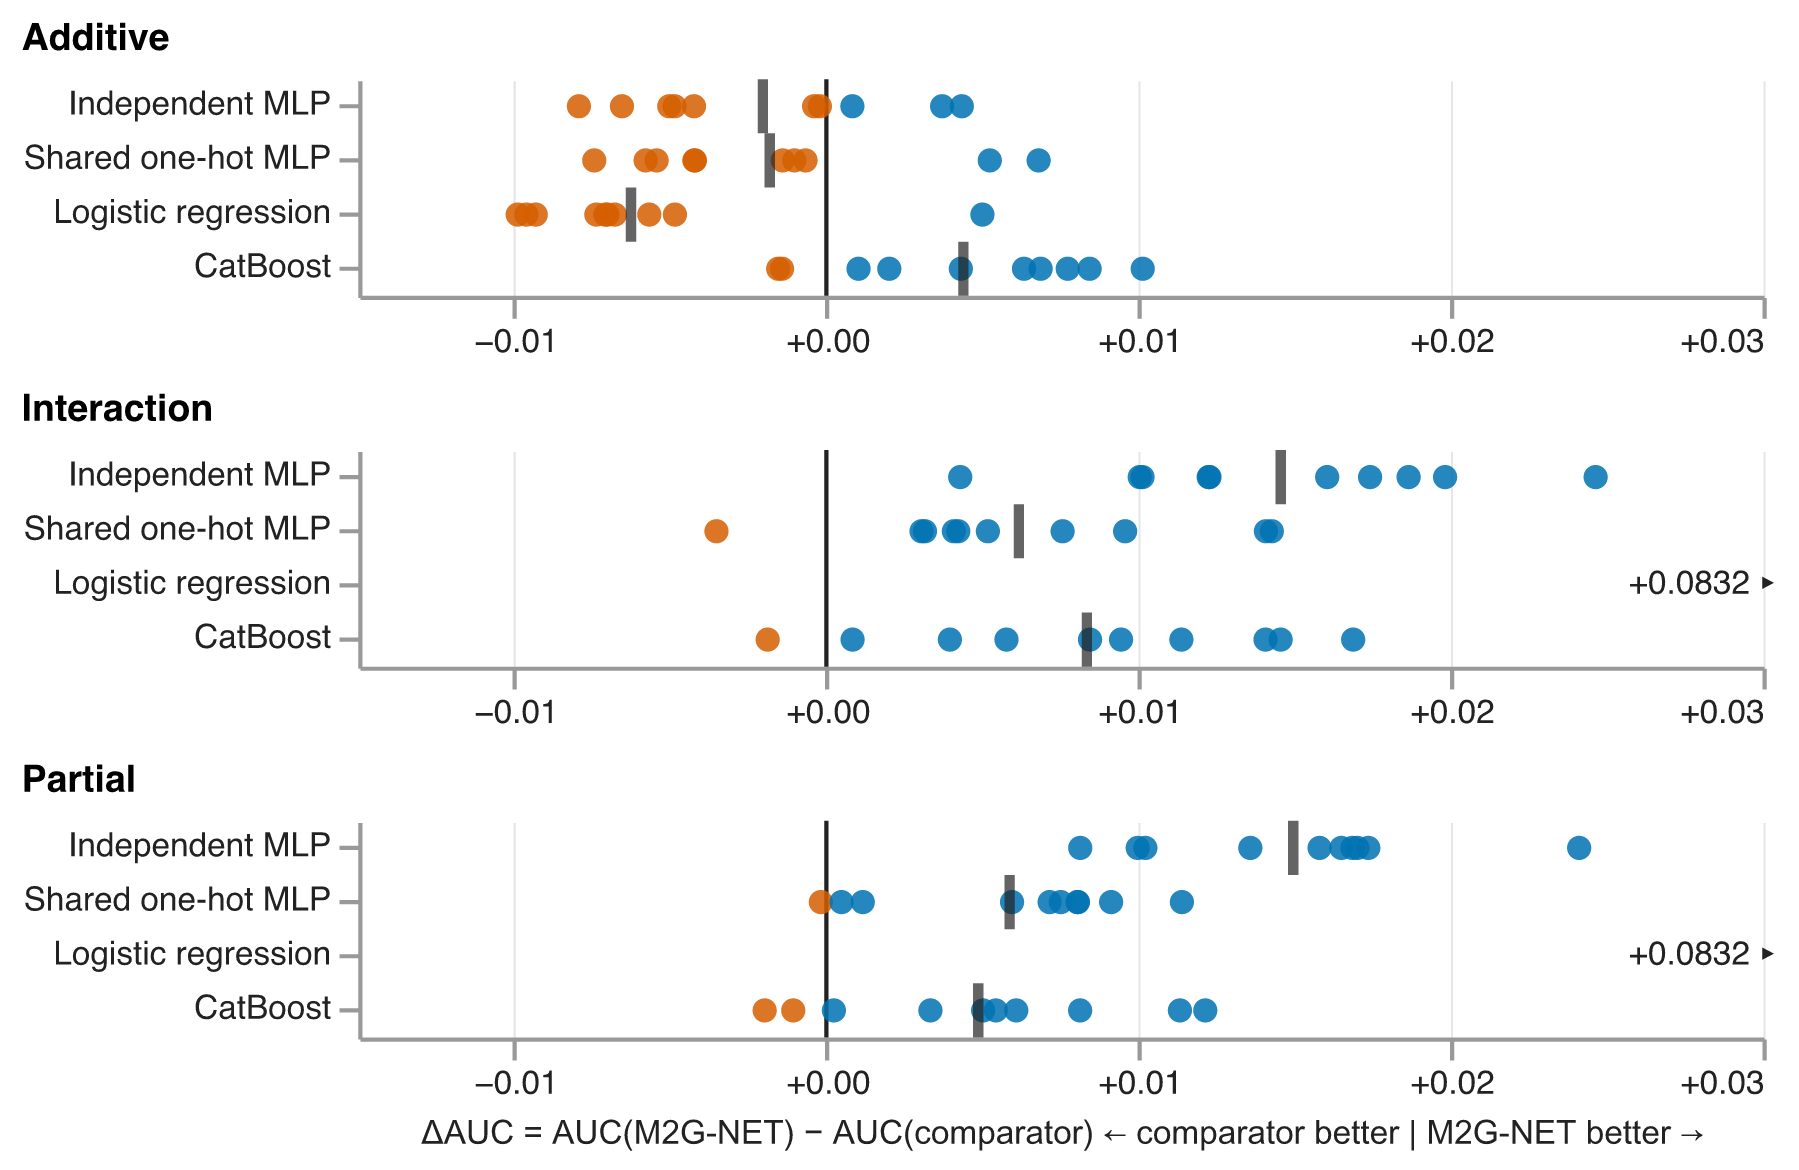
\includegraphics[width=\columnwidth]{figures/fig3_paired_auc.png}
\caption{Paired macro AUC difference, M2G-NET minus comparator, per mechanism. Dots: the ten generated datasets (training-seed averaged); bars: means. Orange favors the comparator, blue favors M2G-NET. Arrows mark comparators whose means lie beyond the axis, printed as means.}
\label{fig:paired}
\end{figure}

\subsection{Execution ceilings}
Extension fits ran four at a time, so their timings are contended and not comparable with Table~\ref{tab:cost}. Parameter counts are not capacity matched across families, so differences cannot be attributed solely to routing, interactions or sharing. All results are descriptive over ten datasets per mechanism conditional on 12 fixed sites; training-seed repeats are not additional independent datasets.

\section{Discussion and Limitations}
\textbf{Answer.} The evaluation supports a bounded answer. In settings with interaction or partial labels M2G-NET was consistently ahead of the independent-head MLP and logistic regression (ten of ten datasets), and usually ahead of CatBoost and the shared one-hot MLP (eight to nine of ten). On additive data simpler references were better. These comparisons do not establish which component, if any, is responsible. The defensible contribution is an audited implementation and a reproducible evaluation with explicit eligibility, observation and scoring populations.

\textbf{Probability quality.} Ranking did not translate into the lowest Brier error. Objectives differ across families (focal scale-weighted surrogate, BCE, native classical losses), so the source of the gap is not isolated, and no calibration benefit is inferred.

\textbf{Limits.} Ten datasets per mechanism were generated, seven of them added post hoc after the first three were examined; the stopping point was therefore data-dependent, and no significance claim is justified. Replicates share 12 fixed sites, so random splitting measures interpolation, not unseen-site transfer. The generator uses fixed categorical laws and a few coefficient settings, with independent outcomes given predictors; it does not test latent dependence, longitudinal effects, continuous covariates or confounding. Capacity, preprocessing and search budgets differ across families, so task sharing, a single product term or routing cannot be isolated. Oracle scoring corrects the evaluation population in this simulation, not a real missing-data process.

\textbf{Transport relevance.} The Hanoi study explains why red-phase and turning encounters need distinct analysis populations \cite{NguyenPhuoc2024same}; it does not validate this generator. No rider prevalence, real behavior, fairness, causal gate explanation or policy follows. An empirical extension would need authorized records, an agreed codebook and eligibility protocol, and site- and time-aware evaluation.

\section{Conclusion}
We audited M2G-NET under synthetic mechanisms with explicit eligibility, partial observation and oracle-isolated scoring. M2G-NET was consistently ahead of independent-head and linear baselines on interaction and partial-label data, simpler procedures won on the additive control, and raw probability error favored other procedures. Ten fixed-site replicates per mechanism, seven added post hoc, are descriptive evidence only; empirical validation would be a separate study.

\textbf{Data and code availability.} All encounters are synthetic and no observational records were obtained. The manuscript and supporting summary artifacts are available at \texttt{github.com/Cuki2910/M2G-NET}. The complete experiment artifacts remain local; publication of this manuscript does not imply that every prediction or execution artifact is included.

\balance
\begin{thebibliography}{20}
\bibitem{NguyenPhuoc2024same} D.~Q. Nguyen-Phuoc, N.~X. Mai, and O.~Oviedo-Trespalacios, ``Not the same: How delivery, ride-hailing, and private riders' roles influence safety behavior,'' \emph{Accid. Anal. Prev.}, vol. 208, 107762, 2024.
\bibitem{RUBIN1976inference} D.~B. Rubin, ``Inference and missing data,'' \emph{Biometrika}, vol. 63, no. 3, pp. 581--592, 1976.
\bibitem{Caruana1997multitask} R.~Caruana, ``Multitask learning,'' \emph{Mach. Learn.}, vol. 28, no. 1, pp. 41--75, 1997.
\bibitem{Misra2016cross} I.~Misra, A.~Shrivastava, A.~Gupta, and M.~Hebert, ``Cross-stitch networks for multi-task learning,'' in \emph{Proc. IEEE CVPR}, 2016, pp. 3994--4003.
\bibitem{Ma2018modeling} J.~Ma, Z.~Zhao, X.~Yi, J.~Chen, L.~Hong, and E.~H. Chi, ``Modeling task relationships in multi-task learning with multi-gate mixture-of-experts,'' in \emph{Proc. ACM SIGKDD}, 2018, pp. 1930--1939.
\bibitem{Tang2020progressive} H.~Tang, J.~Liu, M.~Zhao, and X.~Gong, ``Progressive layered extraction (PLE): A novel multi-task learning model for personalized recommendations,'' in \emph{Proc. ACM RecSys}, 2020, pp. 269--278.
\bibitem{Wang2017deep} R.~Wang, B.~Fu, G.~Fu, and M.~Wang, ``Deep \& cross network for ad click predictions,'' in \emph{Proc. ADKDD}, 2017, pp. 1--7.
\bibitem{Kendall2018multi} A.~Kendall, Y.~Gal, and R.~Cipolla, ``Multi-task learning using uncertainty to weigh losses for scene geometry and semantics,'' in \emph{Proc. IEEE CVPR}, 2018, pp. 7482--7491.
\bibitem{Martins2016from} A.~Martins and R.~Astudillo, ``From softmax to sparsemax: A sparse model of attention and multi-label classification,'' in \emph{Proc. ICML}, PMLR vol. 48, 2016, pp. 1614--1623.
\bibitem{Lin2017focal} T.-Y. Lin, P.~Goyal, R.~Girshick, K.~He, and P.~Doll{\'a}r, ``Focal loss for dense object detection,'' in \emph{Proc. IEEE ICCV}, 2017, pp. 2999--3007.
\bibitem{Morris2019using} T.~P. Morris, I.~R. White, and M.~J. Crowther, ``Using simulation studies to evaluate statistical methods,'' \emph{Stat. Med.}, vol. 38, no. 11, pp. 2074--2102, 2019.
\bibitem{Kingma2015adam} D.~P. Kingma and J.~Ba, ``Adam: A method for stochastic optimization,'' arXiv:1412.6980, 2015.
\bibitem{Prokhorenkova2017catboost} L.~Prokhorenkova, G.~Gusev, A.~Vorobev, A.~V. Dorogush, and A.~Gulin, ``CatBoost: Unbiased boosting with categorical features,'' arXiv:1706.09516, 2017.
\bibitem{Ding2023mitigating} C.~Ding, Z.~Lu, S.~Wang, R.~Cheng, and V.~N. Boddeti, ``Mitigating task interference in multi-task learning via explicit task routing with non-learnable primitives,'' in \textit{Proc. IEEE/CVF CVPR}, 2023, pp. 7756--7765.
\bibitem{Zhang2025bagging} G.-D. Zhang \textit{et al.}, ``Bagging-expert network for multi-task learning: A depolarization solution in multi-gate mixture-of-experts,'' in \textit{Proc. AAAI}, vol. 39, no. 21, 2025, pp. 22389--22397.
\bibitem{Nishi2024joint} K.~Nishi, J.~Kim, W.~Li, and H.~Pfister, ``Joint-task regularization for partially labeled multi-task learning,'' in \textit{Proc. IEEE/CVF CVPR}, 2024, pp. 16152--16162.
\bibitem{Xiao2025explainable} Y.~Xiao and Z.~Duan, ``An explainable multi-task deep learning framework for crash severity prediction using multi-source data,'' \textit{Sci. Rep.}, vol. 15, no. 1, Art. 21978, 2025.
\bibitem{McElfresh2023when} D.~C. McElfresh \textit{et al.}, ``When do neural nets outperform boosted trees on tabular data?'' in \textit{Proc. NeurIPS}, vol. 36, 2023, pp. 76336--76369.
\bibitem{Siepe2024simulation} B.~S. Siepe \textit{et al.}, ``Simulation studies for methodological research in psychology: A standardized template for planning, preregistration, and reporting,'' \textit{Psychol. Methods}, 2024, doi:10.1037/met0000695.
\bibitem{Hardwicke2023reducing} T.~E. Hardwicke and E.-J. Wagenmakers, ``Reducing bias, increasing transparency and calibrating confidence with preregistration,'' \textit{Nat. Hum. Behav.}, vol. 7, no. 1, pp. 15--26, 2023.
\end{thebibliography}

\end{document}
